\subsection{Mini-Batch Gradient Descent}
We saw how vectorization allows us to perform forward and back propagation easily on $m$ training examples. 

$$
X_{(n_x, m)} = \begin{bmatrix}
    \vline &  & \vline\\
    x\idx{1} & \dots & x\idx{m}\\
    \vline &  & \vline
\end{bmatrix}
$$
$$
Y_{(1, m)} = 
\begin{bmatrix}
    y\idx{1} & \dots & y\idx{m}
\end{bmatrix} 
$$

What if $m=5000000$? We split our training set into mini batches of, say $1000$ training samples.
$$
X\ Batches: X\batch{1}, \dots, X\batch{5000}
$$ 
$$
Y\ Batches: Y\batch{1}, \dots, Y\batch{5000}
$$

\begin{itemize}
    \item for $t=1\dots5000$ do:
    \begin{itemize}
        \item[-] Forward Prop on $X\batch{t}$
        \begin{itemize}
            \item[] $Z\lay{1} = W\lay{1}X\batch{t}+b\lay{1}$
            \item[] $A\lay{1} = g\lay{1}(Z\lay{1})$ 
            \item[] $\dots$
            \item[] $Z\lay{L} = W\lay{L}A\lay{L-1}+b\lay{L}$
            \item[] $A\lay{L} = g\lay{L}(Z\lay{L})$ 
        \end{itemize} 
        \item[-] Compute Cost: $J\batch{t}=\frac{1}{1000}\sum{\dots} + \dots$
        \item[-] Back Prop to compute gradients with respect to $J\batch{t}$. 
        \item[-] Update parameters.   
    \end{itemize}
\end{itemize}

\subsection{Understanding Mini-Batch Gradient Descent}

\begin{figure}[H]
    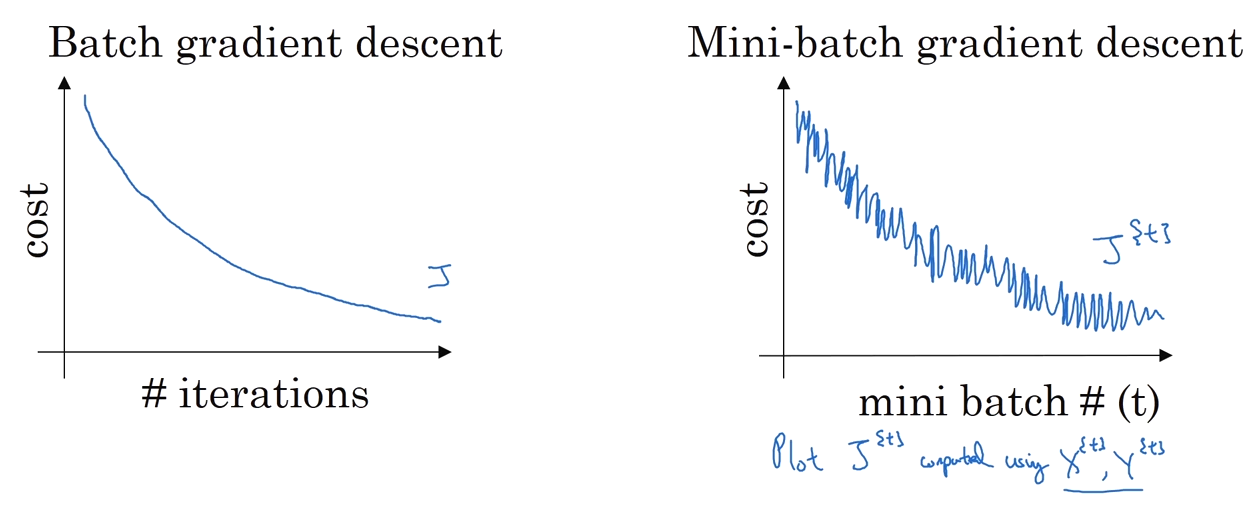
\includegraphics[scale=0.35]{images/minibatch.png}
    \centering
\end{figure}

\begin{itemize}
    \item If mini-batch size equals $m$: Batch Gradient Descent (Blue)
    \item If mini-batch size equals $1$: Stochastic Gradient Descent (Purple)
\end{itemize}

\begin{figure}[H]
    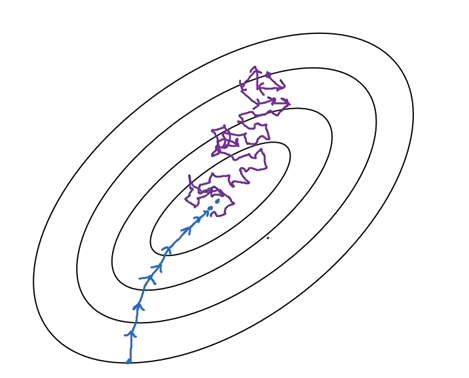
\includegraphics[scale=0.35]{images/stochastic.png}
    \centering
\end{figure}

\textbf{Batch Gradient Descent:} Too long per epoch.

\textbf{Stochastic Gradient Descent:} Losing the speed-up of vectorization. 

\textbf{Somewhere in Between:} Take advantage of the speed-up of vectorization + Make progress without needing to wait. Typical mini-batch sizes are $64, 128, 256, 512$. Make sure your mini-batches fit in CPU/GPU memory. 

\subsection{Exponentially Weighted Averages}
Consider the following example in which we have a sequence of temperatures $\theta_1, \theta_2, \dots$, which is shown by blue dots, and a special average sequence $V$ shown in red: 
\begin{figure}[H]
    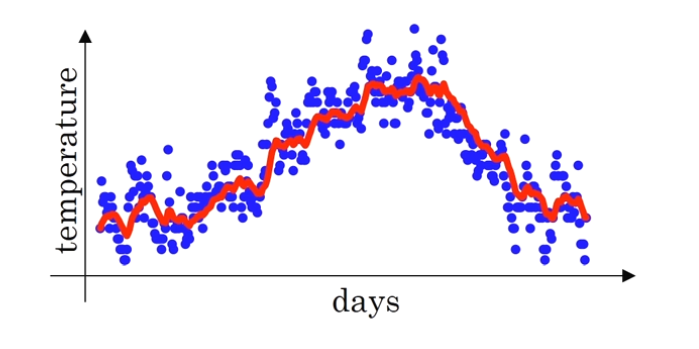
\includegraphics[scale=0.35]{images/avg.png}
    \centering
\end{figure}
Where: 
$$
v_t = \beta v_{t-1} + (1-\beta)\theta_1, \beta = 0.9
$$

It can be shown that the equation above is the approximate average over the last $\approx \frac{1}{1-\beta}$ instances. 

For example, if $\beta=0.98$, we are averaging over $50$ instances. If $\beta=0.5$, we are averaging over $2$ instances. 

\textbf{Understanding Weighted Averages:}
$$
v_{100} = 0.1\theta_{100} + 0.9v_{99}
$$
$$
= 0.1\theta_{100} + 0.9\Big(0.1\theta_{99} + 0.9v_{98}\Big)
$$
$$
= \dots
$$
$$
=0.1\theta_{100} + (0.9)(0.1)\theta_{99} + (0.1)(0.9)^2\theta_{98}+(0.1)(0.9)^3\theta_{97}+\dots
$$

It turns out that all of the coefficients add up to a number very close to $1$. 

If we compute $0.9^10$, we will reach $\approx 0.35 \approx \frac{1}{e}$, which means that after $10$ days, the coefficient will be almost a third of the coefficient of the current thay. 
$$
(1-\epsilon)^{\frac{1}{\epsilon}} \approx \frac{1}{e}
$$

\subsection{Bias Correction of Exponentially Weighted Averages}
For $\beta=0.98$, we would normally expect the green curve. 

\begin{figure}[H]
    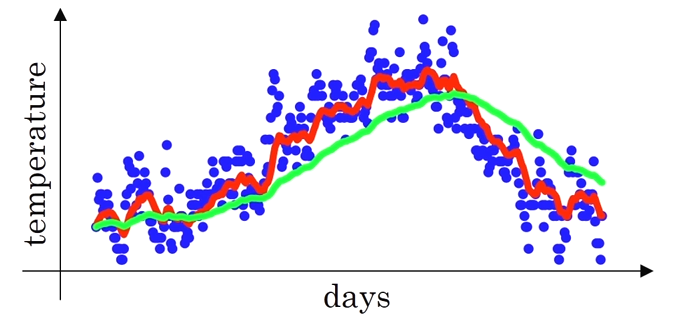
\includegraphics[scale=0.35]{images/green.png}
    \centering
\end{figure}

However, if we implement the formula $v_t = \beta v_{t-1} + (1-\beta)\theta_{t}$, we end up with the purple curve.

\begin{figure}[H]
    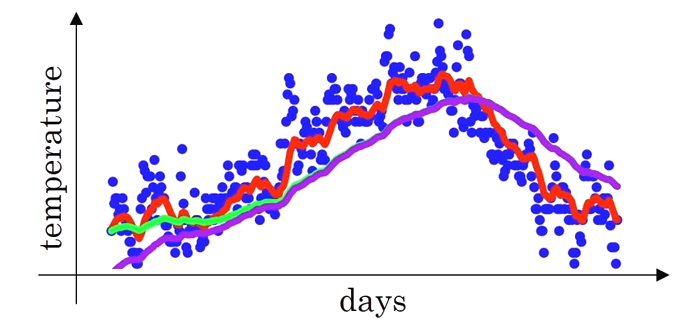
\includegraphics[scale=0.35]{images/purple.png}
    \centering
\end{figure}

This phenomenon is called bias, and it happens because of our initialization of $v_0$, in which we set $v_0=0$. 
 $$
 v_0=0
 $$
 $$
 v_1 = 0.98v_0+0.02\theta_1=0.02\theta_1
 $$
 $$
 v_2 = 0.98v_1+0.02\theta_2 = (0.98)(0.02)\theta_1 + 0.02\theta_2
 $$

 Obviously, our initial $v$s are smaller than expected. What is the remedy to this situation? Instead of calculating $v_t$, we calculate $\frac{v_t}{1-\beta^{t}}$

 $$
 v_2 = \frac{(0.98)(0.02)\theta_1 + 0.02\theta_2}{1-(0.98)^2}
 $$

 We can see that $(0.98)(0.02)=0.0196$ and $0.02$ in the nominator, add up to $1-(0.98)^2 = 0.0396$ in the denominator, making $v_2$ a weighted average of $\theta_1$ and $\theta_2$, thus removing the bias.

This bias correction method helps the purple curve get closer to the green curve.

\subsection{Gradient Descent with Momentum}

Compute an exponentially weighted average of the gradients, and use that to update your parameters. 

The up and down oscillations in gradient descent algorithm prevents us from using a large learning rate, whcih results in the slow convergence of the algorithm. 
\begin{figure}[H]
    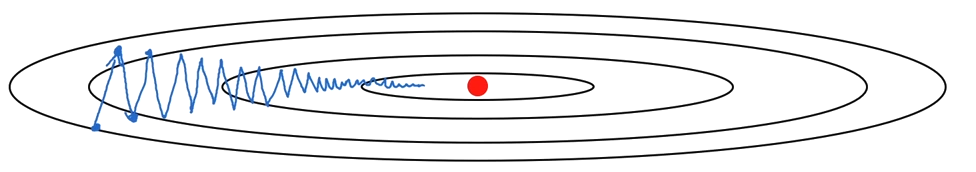
\includegraphics[scale=0.35]{images/GD.png}
    \centering
\end{figure}

\begin{itemize}
    \item On iteration $t$:
    \begin{itemize}
        \item[] Compute $dW, db$ on current mini-batch.
        \item[] $v_{dW} = \beta v_{dW} + (1-\beta)dW$
        \item[] $v_{db} = \beta v_{db} + (1-\beta)db$
        \item[] $W = W - \alpha v_{dW}$, $b = b - \alpha v_{db}$ 
    \end{itemize}
\end{itemize}

We often see this algorithm with the $(1-\beta)$ omitted. 

\subsection{RMSProp}

\begin{itemize} 
    \item On iteration $t$:
    \begin{itemize}
        \item[] Compute $dW, db$ on current mini-batch.
        \item[] $s_{dW} = \beta s_{dW} + (1-\beta)dW^2$, (element-wise)
        \item[] $s_{db} = \beta s_{db} + (1-\beta)db^2$, (element-wise)
        \item[] $W = W - \alpha \frac{dW}{\sqrt{s_{dW}+\epsilon}}$, $b = b - \alpha \frac{db}{\sqrt{s_{db}+\epsilon}}$ 
    \end{itemize}
\end{itemize}

Since we want to reduce the oscillations in vertical ($b$) direction, we are changing our update in a way that horizontal update has greater weight. $s_{dW}$ is relatively small, whereas $s_{db}$ is relatively large. As a result, the updates in the vertical direction are slowed down, whereas updates in the horizontal direction are speeded up. 

More generally, in dimensions where vertical oscillations (oscillations that are not toward the minima) are existent, $s$ will be relatively large, allowing us to use a larger learning rate. 


\subsection{Adam Optimization Algorithm}
It basically takes momentum and RMSProp and puts them together as a new algorithm. 

\begin{itemize} 
    \item On iteration $t$:
    \begin{itemize}
        \item[] Compute $dW, db$ on current mini-batch.
        \item[] Momentum with $\beta_1$: $$v_{dW} = \beta_1 v_{dW} + (1-\beta_1)dW$$ $$v_{db} = \beta_1 v_{db} + (1-\beta_1)db$$
        \item[] RMSProp with $\beta_2$: $$s_{dW} = \beta_2 s_{dW} + (1-\beta_2)dW^2$$ $$s_{db} = \beta_2 s_{db} + (1-\beta_2)db^2$$
        \item[] Perform bias correction: 
        $$v^{corrected}_{dW} = \frac{v_{dW}}{1-\beta_1^t}$$ 
        $$v^{corrected}_{db} = \frac{v_{db}}{1-\beta_1^t}$$ 
        $$s^{corrected}_{dW} = \frac{s_{dW}}{1-\beta_2^t}$$ 
        $$s^{corrected}_{db} = \frac{s_{db}}{1-\beta_2^t}$$ 
        \item[] Update parameters: 
        $$W = W - \alpha\frac{v^{corrected}_{dW}}{\sqrt{s^{corrected}_{dW} + \epsilon}}$$ 
        $$b = b - \alpha\frac{v^{corrected}_{db}}{\sqrt{s^{corrected}_{db} + \epsilon}}$$ 
    \end{itemize}
\end{itemize}

\begin{itemize}
    \item $\alpha$: Needs to be tuned
    \item $\beta_1$ = $0.9$
    \item $\beta_2$ = $0.999$
    \item $\epsilon$ = $10^{-8}$
\end{itemize}

\subsection{Learning Rate Decay}
Smaller learning rates tend to wander around tighter regions around the minimum. As a result, it is intuitive that we slow down our learning with the passage of time.

We know that 1 epoch means 1 pass through the data. 

$$
\alpha = \frac{1}{1 + decayRate * epoch} \alpha_0
$$

There are other decay methods too: 
$$
\alpha = (0.95)^{epoch} \alpha_0
$$
$$
\alpha = \frac{k}{\sqrt{epoch}}\alpha_0
$$